\subsection{$D$ and $B$ mesons}

Heavy flavor quark ($c$ and $b$) production in pPb collisions
can be well explored over a wide transverse momentum range
in a high-luminosity run in 2016. 


\begin{figure}[h]
\begin{center}
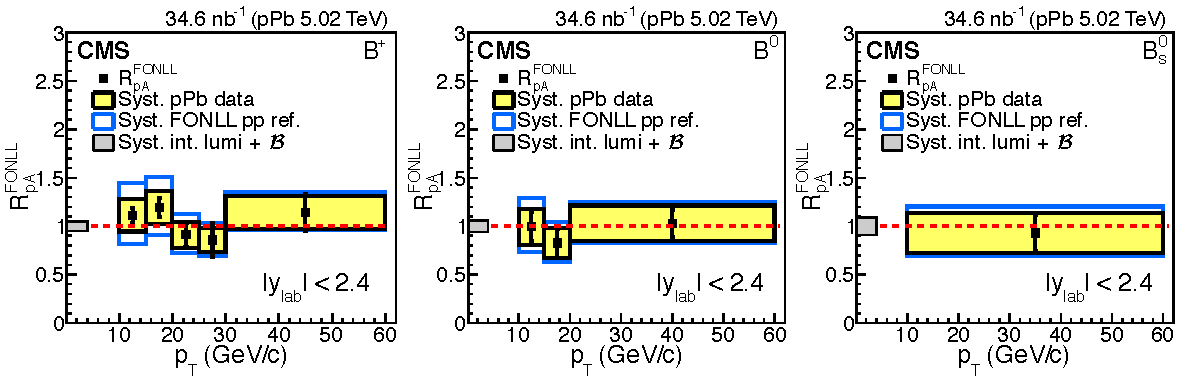
\includegraphics[width= 0.95\textwidth]{figures/nuclearmodification.pdf}
\caption{Nuclear modification factor in pPb collisions at \rootsNN\ = 5.02 TeV 
obtained with L$_{\rm int}$ = 35 nb$^{-1}$~\cite{PhysRevLett.116.032301}.}
\label{fig:measurementB}
\end{center}
\end{figure}


At low \pt, the study of the nuclear modification factors of
$D$ and $B$ mesons allows to test the relevance of cold nuclear matter 
effects in the heavy flavor sector, 
as predicted in Refs.~\cite{Eskola:2009uj,deFlorian:2003qf,Frankfurt:2011cs}. 
Gluon saturation processes are expected to reduce the production 
cross sections of $D$ mesons by about 10--20\% at \pt\ about 2--3 GeV/c.  
In the $B$ sector, a smaller modification comparing to that for 
$D$ mesons is expected as a consequence of the larger $x$ range 
covered at a similar \pt\ range. A precise measurement of the $D$ and $B$ 
nuclear modification factors in pPb collisions at low \pt\ is therefore 
needed to experimentally validate the theoretical expectations. 


\begin{figure}[h]
\begin{center}
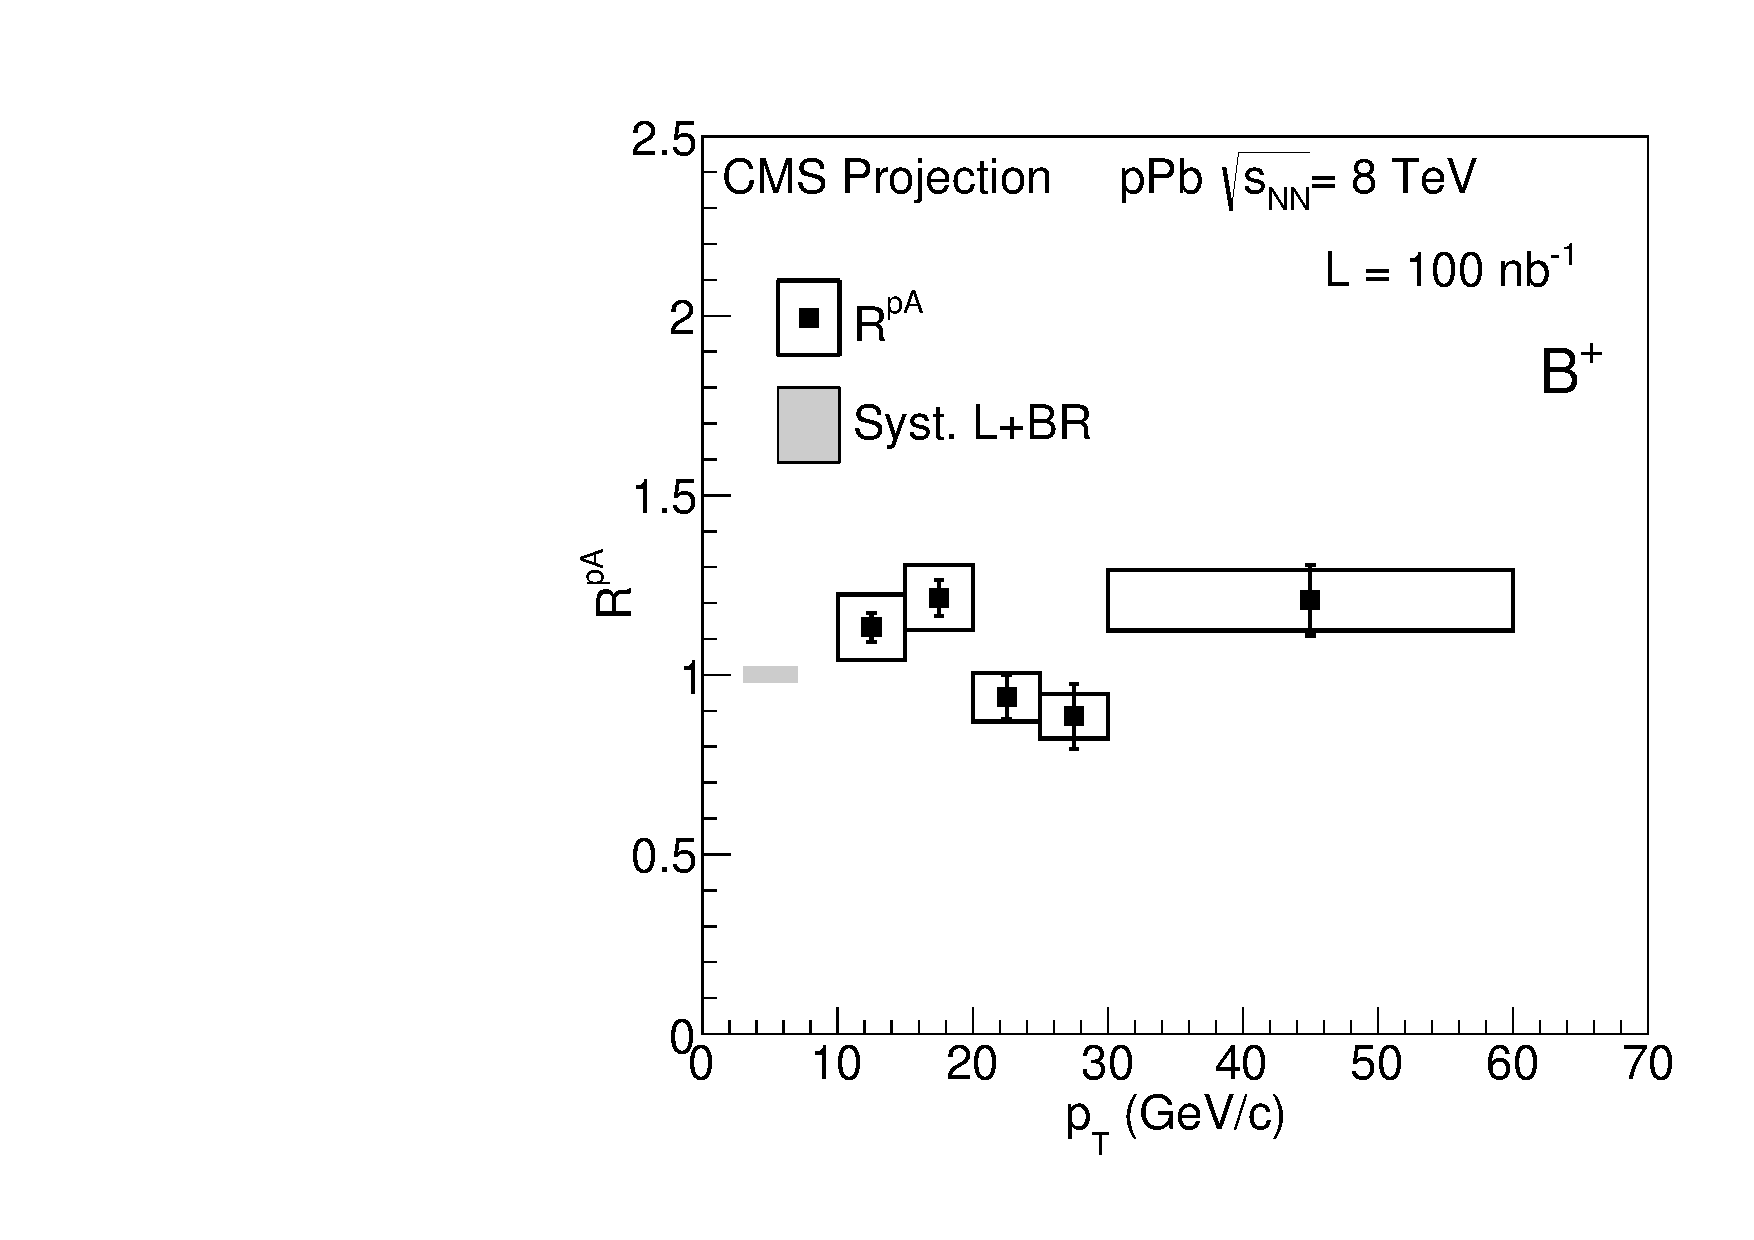
\includegraphics[width= 0.55\textwidth]{figures/canvasrpabplus}
\caption{Projected $\rm B^{+}$ meson $\rm R_{pPb}$ estimated for pPb collisions at \rootsNN\ = 8.16 TeV 
with L$_{\rm int}$ = 100 nb$^{-1}$ based on 2011 pPb measurement.}
\label{fig:Bextrapolated}
\end{center}
\end{figure}

In Fig.~\ref{fig:measurementB}, CMS measurement of nuclear modification factors
for $B$ mesons in pPb collisions at \rootsNN\ = 5.02 TeV with L$_{\rm int}$ = 35 nb$^{-1}$ 
is presented~\cite{PhysRevLett.116.032301}. The current statistical 
and systematic uncertainties do not allow to conclude any significant 
deviation from unity. In Fig.~\ref{fig:Bextrapolated}, the result expected 
at \rootsNN\ = 8.16 TeV considering an integrated luminosity of 100 nb$^{-1}$ 
is presented. In order to have the possibility to measure $B$ meson 
production down to very low \pt\ with the needed accuracy (~5--10\%), 
the highest possible integrated luminosity is therefore necessary in 2016 run.

\begin{figure}[h]
\begin{center}
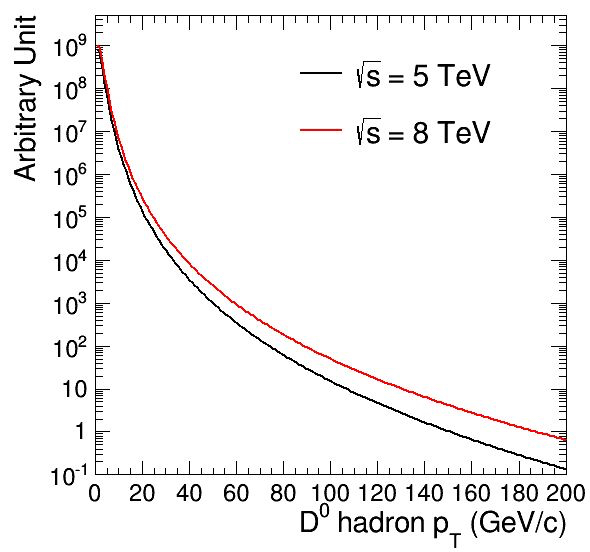
\includegraphics[width= 0.45\textwidth]{figures/D-Sigma.jpg}
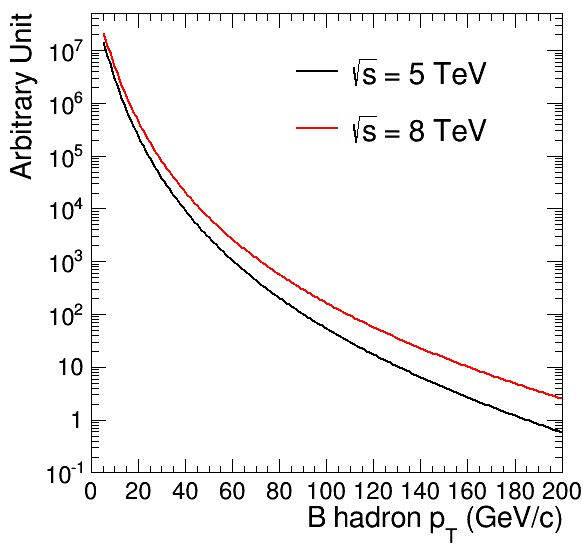
\includegraphics[width= 0.45\textwidth]{figures/B-Sigma.jpg}
\caption{FONLL predictions for $D$ (left) and $B$ (right) meson production 
in pp collisions at \roots\ = 8.16 and 5.02 TeV as a function of \pt\ ~\cite{FONLLcharmbottomPP1}.
The unit of y axis is arbitrary.
}
\label{fig:plotsDBpredictions}
\end{center}
\end{figure}

Meanwhile, a large pPb data sample would also be beneficial for 
studying heavy flavor production at very high \pt\ to explore
nuclear modification effect in a larger $x$ ranger. 
In Fig.~\ref{fig:plotsDBpredictions}, the FONLL predictions 
for $D$ (left) and $B$ (right) cross sections (with arbitrary unit) 
in pp collisions are shown as a function of \pt\ for both \roots\ = 5.02 and 8.16 TeV.
A factor of about 2 increase in heavy-flavor cross section is
expected at \pt\ $\approx$ 100 GeV/c as a consequence of higher
collision energy. Assuming an integrated luminosity of 100~nb$^{-1}$
for 2016 pPb sample, a factor of 6 increase of heavy-flavor signals
is expected.